\documentclass{beamer}

\usepackage{beamerthemesplit}
\usetheme{Singapore} 

\input{../../include/preamble.inc} 
\input{../../include/definitions.inc} 
\input{../../include/author.inc} 

\title[]{Законы сохранения в механике сплошных сред}

\begin{document}
	
\frame[plain]{\titlepage}


\frame[plain]{
	\frametitle{Аннотация}
	\parbox{\textwidth}{
	Траектрория движения сплошной среды. Формула Эйлера. Законы сохранения параметров сплошной среды в интегральной и дифференциальной форме. 
	}
}

\frame{
	\frametitle{ Траектории движения точек и теорема об определителе }
	
		\begin{columns}
			\begin{column}{0.45\textwidth}
				\centering
				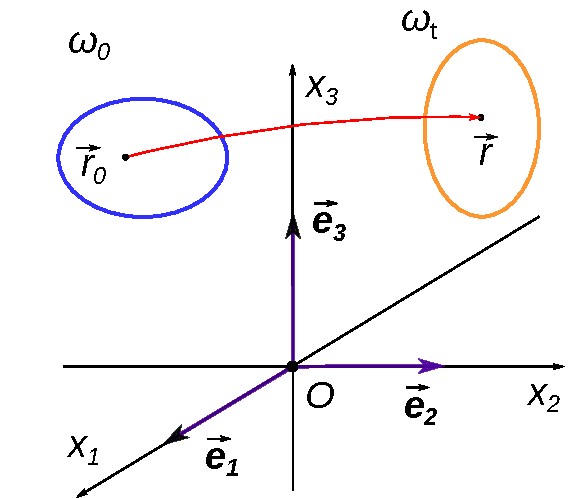
\includegraphics[width=\textwidth]{../img/omega_def.pdf}	
			\end{column}
			\begin{column}{0.55\textwidth}
%				\scriptsize
				\begin{exampleblock}{Иллюстрация перемещения сплошной среды}
					\parbox{\textwidth}{
					$\omega_0$, $\omega_t$ -- положение части сплошной среды в начальный момент времени и момент $t$.
					\[
					\vec{r}_0 = \xi^1\vec{e}_1+\xi^2\vec{e}_2+\xi^3\vec{e}_3,
					\]
					\[
					\vec{r} = x^1\vec{e}_1+x^2\vec{e}_2+x^3\vec{e}_3.
					\]
				}
				\end{exampleblock}				
			\end{column}
		\end{columns}
	

		\begin{exampleblock}{Траектории движения}
			\parbox{\textwidth}{
				Траектории движения жидких частиц задаются функцией
				\[
					\vec{x} = \vec{x} \argtxi,
				\]
				где $\vec{\xi}$, $\vec{x}$ -- лагранжевы и эйлеровы координаты частицы.
			}
		\end{exampleblock}
}

\frame{
	\frametitle{ Определение траекторий по заданному полю движения }
		\begin{exampleblock}{Поле скоростей}
			\parbox{\textwidth}{
				Поле скоростей частиц сплошной среды в эйлеровой системе координат задается функцией $\vec{v}\argtx$. В лагранжевой системе координат скорость определяется соотношением
				\[
				\vec{v}\argtxiv = \pd{\vec{x} \argtxiv}{t}.
				\]
			}
		\end{exampleblock}

%					\vec{v} = \vec{v} \argtx

		\begin{exampleblock}{Задача определения траекторий движения по заданному полю скоростей}
		\parbox{\textwidth}{
			По заданному полю скоростей $\vec{v}\argtxv$ требуется найти траектории движения частиц $x^i = x^i\argtxiv$ с лагранжевыми координатами $\argxiv$:
			\[
			\pd{x^i}{t} = v^i\argtxv,\quad
			x^i |_{t=0} = \xi^i\quad
			(i=1,2,3).
			\]	
		}
	\end{exampleblock}
}

\frame{
	\frametitle{ Уравнения для нахождения матрицы Якоби }
	
	\begin{exampleblock}{Матричное уравнение для нахождения матрицы Якоби}
		\parbox{\textwidth}{
			Дифференцируя уравнения для нахождения траекторий по $\xi^j$, получим:
			\[
			\pd{}{t} \pd{x^i}{\xi^j} = \pd{v^i}{x^k}\pd{x^k}{\xi^j},\quad
			\left. \pd{x^i}{\xi^j} \right|_{t=0}=\delta^i_j.
			\]
			
			Тогда матрица Якоби $y_{ij} = \displaystyle\pd{x^i}{\xi^j}$ удовлетворяет дифференциальному уравнению:
			\[
			\pd{Y}{t}=AY,\quad Y|_{t=0} = E,
			\]
			где $A$ -- матрица, составленная из производных $\displaystyle\pd{v^i}{x^j}$; $E$ -- единичная матрица.
		}
	\end{exampleblock}
	
}

\frame{
	\frametitle{ Геометрический смысл определителя }
	
	
	\begin{columns}
		\begin{column}{0.5\textwidth}
			\centering
			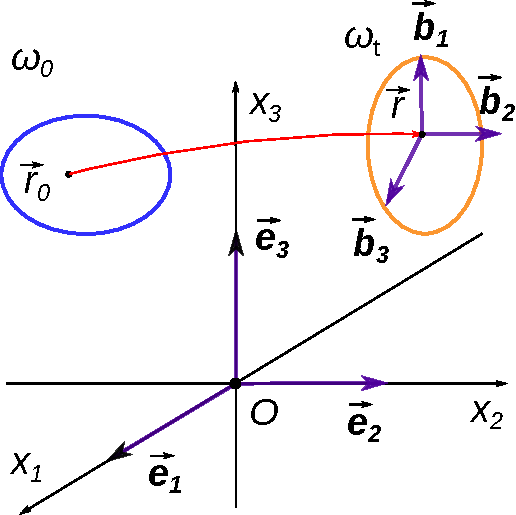
\includegraphics[width=\textwidth]{../img/omega_def_bi.pdf}		
		\end{column}
		\begin{column}{0.5\textwidth}
			\begin{exampleblock}{Сопутствующий базис}
				\parbox{\textwidth}{
					\[
					\vec{b}_i = \pd{\vec{r}}{\xi^i} = \pd{x^j}{\xi^i}\vec{e}_j
					\]
				}
				\begin{exampleblock}{Элементарный объем}
					\parbox{\textwidth}{ 
						\[
						\Delta\argtxiv =
						\left|\displaystyle
						\begin{array}{ccc}
						\displaystyle\pd{x^1}{\xi^1} & \displaystyle\pd{x^2}{\xi^1} & \displaystyle\pd{x^3}{\xi^1} \\
						\displaystyle\pd{x^1}{\xi^2} & \displaystyle\pd{x^2}{\xi^2} & \displaystyle\pd{x^3}{\xi^2} \\	\displaystyle\pd{x^1}{\xi^3} & \displaystyle\pd{x^2}{\xi^3} & \displaystyle\pd{x^3}{\xi^3}				
						\end{array}
						\right|=
						\]
						\[
						= \vec{b}_1 \cdot (\vec{b}_2 \times \vec{b}_3)
						\]
						
					}
				\end{exampleblock}
			\end{exampleblock}
		\end{column}
	\end{columns}
	
	
	
	
	
}

\frame{
	\frametitle{ Дифференцирование определителя матрицы Якоби }
	\parbox{\textwidth}{
	
		Обозначим $\Delta\argtxiv = \operatorname{det} Y\argtxiv$, тогда из формулы определителя как суммы произведений его элементов и правила дифференцирования произведения имеем:
		\[
		\Delta'(t) = \pd{}{t} 
		\left|
		\begin{array}{ccc}
		y_{11} & y_{12} & y_{13} \\
		y_{21} & y_{22} & y_{23} \\
		y_{31} & y_{32} & y_{33} \\
		\end{array}
		\right|=
		\]
		\[
		=		\left|
		\begin{array}{ccc}
		y'_{11} & y'_{12} & y'_{13} \\
		y_{21} & y_{22} & y_{23} \\
		y_{31} & y_{32} & y_{33} \\
		\end{array}
		\right|+
				\left|
		\begin{array}{ccc}
		y_{11} & y_{12} & y_{13} \\
		y'_{21} & y'_{22} & y'_{23} \\
		y_{31} & y_{32} & y_{33} \\
		\end{array}
		\right|+
				\left|
		\begin{array}{ccc}
		y_{11} & y_{12} & y_{13} \\
		y_{21} & y_{22} & y_{23} \\
		y'_{31} & y'_{32} & y'_{33} \\
		\end{array}
		\right|.
		\]
	}
	
}

\frame{
	\frametitle{ Дифференцирование определителя матрицы Якоби }

	\parbox{\textwidth}{
		Из матричного уравнения $\displaystyle\frac{dY}{dt}=AY$ следует, что
		\[
		y'_{1j} = a_{11}y_{1j}+a_{12}y_{2j} + a_{13}y_{3j},
		\]
		поэтому
		\[
		(y'_{11}, y'_{12}, y'_{13}) = a_{11}(y_{11}, y_{12}, y_{13})+
		a_{12}(y_{21}, y_{22}, y_{23})+
		a_{13}(y_{31}, y_{32}, y_{33}).
		\]
		Отсюда, вычитая из первой строки с производными линейную комбинацию остальных строк, получаем:
		\[
		\left|
		\begin{array}{ccc}
			y'_{11} & y'_{12} & y'_{13} \\
			y_{21} & y_{22} & y_{23} \\
			y_{31} & y_{32} & y_{33} \\
		\end{array}
		\right|=
		\left|
		\begin{array}{ccc}
		a_{11} y_{11} & a_{11} y_{12} & a_{11} y_{13} \\
		y_{21} & y_{22} & y_{23} \\
		y_{31} & y_{32} & y_{33} \\
		\end{array}
		\right|=
		a_{11} \Delta(t).
		\]


	}


	
}

\frame{
	\frametitle{ Дифференцирование определителя матрицы Якоби }
	
	По аналогии можно получить, что
	\[
	\left|
	\begin{array}{ccc}
	y_{11} & y_{12} & y_{13} \\
	y'_{21} & y'_{22} & y'_{23} \\
	y_{31} & y_{32} & y_{33} \\
	\end{array}
	\right| = a_{22} \Delta(t),\quad
	\left|
	\begin{array}{ccc}
	y_{11} & y_{12} & y_{13} \\
	y_{21} & y_{22} & y_{23} \\
	y'_{31} & y'_{32} & y'_{33} \\
	\end{array}
	\right|=a_{33}\Delta(t).
	\]
	
	
	Таким образом,
	\[
	\Delta'(t) = (a_{11}+a_{22}+a_{33}) \Delta(t)=\operatorname{tr} A \, \Delta(t).
%	=	\pd{v^i}{x^i}\Delta(t) = \Delta(t) \operatorname{div} \vec{v} 
	\]
	
	\begin{exampleblock}{Правило дифференцирования определителя матрицы Якоби, или формула Эйлера}
		\medskip
		\parbox{\textwidth}{
			\[
			\pd{}{t}\left| \pd{x^i}{\xi^j} \right| = \left| \pd{x^i}{\xi^j} \right|
			\left(
			\pd{v^1}{x^1}+\pd{v^2}{x^2}+\pd{v^3}{x^3}
			\right)=
			 \left| \pd{x^i}{\xi^j} \right|\operatorname{div} \vec{v}
			\]
		}
	\end{exampleblock}
	
}

\frame{
	\frametitle{ Закон дифференцирования интеграла, зависящего от времени }
	\begin{exampleblock}{Упрощения}
		\parbox{\textwidth}{
		\[
		\frac{d}{dt}\int\limits_{\omega_t} F\argtxv  d\vec{x}=
		\frac{d}{dt}\int\limits_{\omega_0} F\argtxiv \Delta\argtxiv d\vec{\xi}=
		\int\limits_{\omega_0} \pd{}{t}(F\argtxiv \Delta\argtxiv) d\vec{\xi}=
		\]
		\[
		=
		\int\limits_{\omega_0} \left( \pd{F\argtxiv }{t}\Delta\argtxiv + F\argtxiv\pd{\Delta\argtxiv}{t} \right) d\vec{\xi} =
		\]
		\[
		=
		\int\limits_{\omega_0} \left( \pd{F\argtxiv }{t} + F\argtxiv \operatorname{div}_{\xi}\vec{v}\argtxiv \right)\Delta\argtxiv  d\vec{\xi} =
		\]
		\[
		=
		\int\limits_{\omega_t} \left( \pd{F\argtxv }{t} + \pd{F\argtxv}{x^i} v^i\argtxv + F\argtxv \operatorname{div}_{x}\vec{v}\argtxv \right)  d\vec{x}
		\]
		}
	\end{exampleblock}
	
}

\frame{
	\frametitle{Закон дифференцирования интеграла, зависящего от времени }
%		\begin{exampleblock}{Упрощения}
%		\parbox{\textwidth}{
%			\[
%			=
%			\int\limits_{\omega_t} \left( \pd{F\argtxv }{t} + \pd{F\argtxv}{x^i} v^i\argtxv + F\argtxv \operatorname{div}_{x}\vec{v}\argtxv \right)  d\vec{x}.
%			\]
%
%		}
%	\end{exampleblock}
	\begin{exampleblock}{Окончательный вид}
		\parbox{\textwidth}{
			\[
			\frac{d}{dt}\int\limits_{\omega_t} F\argtxv  d\vec{x}=
			\int\limits_{\omega_t} \left( \frac{dF\argtxv }{dt}  + F\argtxv \operatorname{div}_{x}\vec{v}\argtxv \right)  d\vec{x},
			\]
			где $d/dt$ -- оператор полного дифференцирования в правой части равенства, который задается формулой:
			\[
				\frac{d}{dt}=\pd{}{t} + (\vec{v}\cdot\nabla).
			\]
			
			
		}
	\end{exampleblock}

	\begin{exampleblock}{Упрощения}
		\parbox{\textwidth}{
			Легко показать, что для $F=F\argtxv$, $\vec{v}=\vec{v}\argtxv$:
			\[
			\frac{dF}{dt}  + F \operatorname{div}\vec{v} = \pd{F}{t} + \operatorname{div} (F\vec{v}).
			\]
			
			
		}
	\end{exampleblock}
}



\frame{
	\frametitle{ Закон сохранения массы сплошной среды }
	\begin{columns}
		\begin{column}{0.45\textwidth}
			\centering
			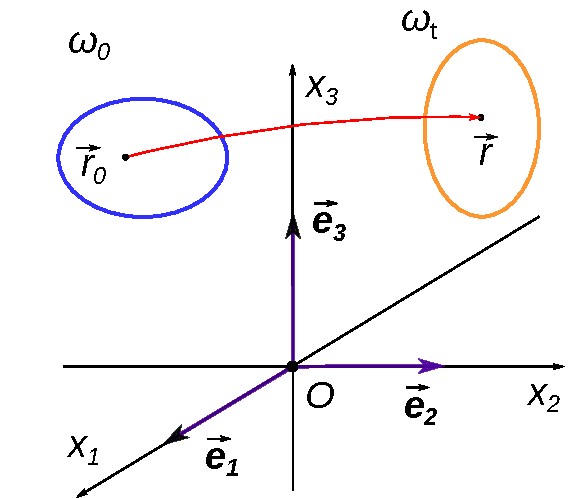
\includegraphics[width=\textwidth]{../img/omega_def.pdf}	
		\end{column}
		\begin{column}{0.55\textwidth}
			\begin{exampleblock}{Интегральный вид ЗСМ}
				\parbox{\textwidth}{
					\[
					\frac{d}{dt}\int\limits_{\omega_t}\rho\argtxv d\vec{x} = 0,				
					\]
					где $\rho\argtxv$ -- плотность жидкой частицы в точке $\vec{r}$ в момент времени $t$.
				}
			\end{exampleblock}		
		\end{column}
	\end{columns}
	
	
		\begin{exampleblock}{Дифференциальная форма}
		\parbox{\textwidth}{
			\begin{tabular}{p{0.5\textwidth}|p{0.5\textwidth}}
				\em	Консервативная & \em	 Неконсервативная \\
				\hline
				&   \\
				$
				\displaystyle\pd{\rho}{t} + \operatorname{div} (\rho \vec{v}) = 0
				$
				& 
				$
				\displaystyle\frac{d\rho}{dt} + \rho \operatorname{div}\vec{v} = 0
				$
			\end{tabular}
		}
	\end{exampleblock}
}

\frame{
	\frametitle{ Закон сохранения импульса сплошной среды }
	
	\begin{exampleblock}{Интегральная форма}
		\parbox{\textwidth}{
		\[
		\frac{d}{dt}\int\limits_{\omega_t}\rho \vec{v} \, d\vec{x} = \int\limits_{s_t}	\vec{\sigma}_n dS + \int\limits_{\omega_t}\rho \vec{f} \, d\vec{x},
		\]
		где $\rho\argtxv$, $\vec{v}\argtxv$ -- плотность и скорость материальной точки сплошной среды; $\vec{\sigma}_n\argtxv$ -- напряжение, возникающее на обозначенной $s_t$ поверхности объема $\omega_t$, на площадке с внешней единичной нормалью $\vec{n}$; $\vec{f}\argtxv$ -- массовая сила, действующая на сплошную среду.
		}
	\end{exampleblock}

	\begin{exampleblock}{Дифференциальная форма}
		\parbox{\textwidth}{
			\begin{tabular}{p{0.5\textwidth}|p{0.5\textwidth}}
			\em	Консервативная & \em	 Неконсервативная \\
			\hline
				&   \\
			$
			\displaystyle\pd{\rho\vec{v}}{t} + \operatorname{div} (\rho\vec{v}\otimes\vec{v} - \sigma) = \rho\vec{f} 	
			$
			& 
			$
			\rho\displaystyle\frac{d\vec{v}}{dt} - \operatorname{div} \sigma = \rho\vec{f} 	
			$
			\end{tabular}
		}
	\end{exampleblock}
}

\frame{
	\frametitle{ Закон сохранения момента импульса сплошной среды }
	
	\begin{exampleblock}{Интегральная форма}
		\parbox{\textwidth}{
			\[
			\frac{d}{dt}\int\limits_{\omega_t} \left(\rho \vec{v}\times\vec{x} +\rho \vec{k} \right) \, d\vec{x} = \int\limits_{s_t}	\vec{\sigma}_n \times\vec{x} \, dS+ \int\limits_{\omega_t}\rho \vec{f} \times\vec{x} \, d\vec{x}+
			\]
			\[	+
				\int\limits_{\omega_t}\rho \vec{h}  \, d\vec{x} +
				\int\limits_{\omega_t} \vec{M}_n dS,
			\]
			где $\rho\argtxv$, $\vec{v}\argtxv$ -- плотность и скорость материальной точки сплошной среды; $\vec{\sigma}_n\argtxv$ -- напряжение, возникающее на обозначенной $s_t$ поверхности объема $\omega_t$,  на площадке с внешней единичной нормалью $\vec{n}$; $\vec{f}\argtxv$ -- массовая сила, действующая на сплошную среду; $\vec{k}$ -- плотность собственного момента количества движения; $\vec{h}$, $\vec{M}_n$ -- плотность массовых и поверхностных пар.
		}
	\end{exampleblock}

	\begin{exampleblock}{Предположения}
		\parbox{\textwidth}{
			\[
				\vec{k} = \vec{h} = \vec{0} ,\quad \vec{M}_n = \vec{0}.
			\]
			
		}
	\end{exampleblock}
	

}



\frame{
	\frametitle{ Следствия закона сохранения момента импульса }

	\begin{exampleblock}{Дифференциальная форма}
		\parbox{\textwidth}{
		\[
		\frac{d}{dt} \left(\rho\vec{v}\times\vec{x}\right) + 	
		(\rho\vec{v}\operatorname{div} \vec{v}) \times\vec{x}  - 
		\operatorname{div} \left(\sigma\times \vec{x}\right) =
		\rho\vec{f}\times \vec{x}
		\]
		}
	\end{exampleblock}


	\begin{exampleblock}{Упрощения}
		\parbox{\textwidth}{
			\[
				\frac{d}{dt} \left(\rho\vec{v}\times\vec{x}\right)	= 
				\frac{d}{dt} (\rho\vec{v}) \times \vec{x} + 
				\rho\vec{v} \times\frac{d\vec{x}}{dt} =
				\frac{d (\rho\vec{v})}{dt} \times \vec{x}
			\]
			\[
				\operatorname{div} \left(\sigma\times \vec{x}\right) = 
				\pd{}{x_i} (\vec{\sigma}_i \times \vec{x}) = 
				\pd{\vec{\sigma}_i}{x_i}\times \vec{x}+\vec{\sigma}_i \times \pd{\vec{x}}{x_i}=
				\operatorname{div} \sigma \times\vec{x}+
				\vec{\sigma}_i \times \vec{e}_i
			\]
		}
	\end{exampleblock}

	\begin{exampleblock}{Упрощение закона сохранения момента импульса}
		\parbox{\textwidth}{
			Умножая векторно закон сохранения импульса на $\vec{x}$ и вычитая из дифференциальной формы с учетом проделанных операций, имеем:
			\[
			\vec{\sigma}_1  \times \vec{e}_1 + \vec{\sigma}_2  \times \vec{e}_2 + \vec{\sigma}_3 \times \vec{e}_3 = \vec{0}.
			\]
			
		}
	\end{exampleblock}


%	\begin{exampleblock}{Следствие}
%	\parbox{\textwidth}{
%		Симметричность тензора напряжений
%		\[
%		\sigma^* = \sigma.
%		\]
%	}
%\end{exampleblock}	
}



\frame{
	\frametitle{ Следствия закона сохранения момента импульса  }
	
	
	\begin{columns}
		\begin{column}{0.75\textwidth}\
			\parbox{\textwidth}{
			
			Упростим равенство:
			\[
			\vec{\sigma}_1  \times \vec{e}_1 + \vec{\sigma}_2 \times  \vec{e}_2 + \vec{\sigma}_3 \times \vec{e}_3 = \vec{0}.
			\]
			
			\[+
				\begin{array}{ccc}
					\sigma_{1j}\vec{e}_j \times \vec{e}_1 & = & -\sigma_{12}\vec{e}_3+\sigma_{13}\vec{e}_2\\
					\sigma_{2j}\vec{e}_j \times \vec{e}_2 & = & \sigma_{21}\vec{e}_3 - \sigma_{23} \vec{e}_1\\
					\sigma_{3j}\vec{e}_j \times \vec{e}_3 & = & -\sigma_{31}\vec{e}_2 + \sigma_{32} \vec{e}_1\\
					\hline
					\vec{\sigma}_i\times\vec{e}_i & = & 
					(\sigma_{32}-\sigma_{23})\vec{e}_1 + \\
					& & +
					(\sigma_{13}-\sigma_{31})\vec{e}_2 +\\
					& & +
					(\sigma_{21}-\sigma_{12})\vec{e}_3.
				\end{array}
			\]
							
			}
		\end{column}
		\begin{column}{0.25\textwidth}
			\centering
			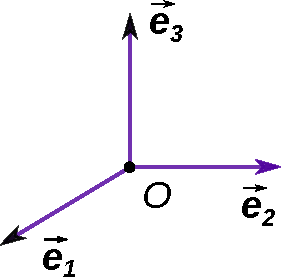
\includegraphics[width=\textwidth]{../img/orth.pdf}
			
			\begin{eqnarray*}
				\vec{e}_1\times\vec{e}_2 &  = &  \vec{e}_3,\\
				\vec{e}_2\times\vec{e}_3 &  = &  \vec{e}_1,\\
				\vec{e}_3\times\vec{e}_1 &  = &  \vec{e}_2.
			\end{eqnarray*}
			
			
		\end{column}
		
	\end{columns}

	\begin{exampleblock}{Симметричность тензора напряжений}
		\parbox{\textwidth}{
			При отсутствии собственного момента количества движения среды и массовых и поверхностных пар имеет место симметричность тензора напряжений:
			\[
			\sigma_{ij} = \sigma_{ji}.
			\]
		}
	\end{exampleblock}
}


\frame{
	\frametitle{ Закон сохранения энергии сплошной среды }
	
	\begin{exampleblock}{Интегральная форма}
		\parbox{\textwidth}{
			\[
			\frac{d}{dt}\int\limits_{\omega_t}\rho \left(\varepsilon + \frac{\vec{v}^2}{2}\right) \, d\vec{x} = \int\limits_{s_t} (\vec{\sigma}_n\cdot\vec{v})\,dS - \int\limits_{s_t} (\vec{q}\cdot\vec{n}) \, dS + \int\limits_{\omega_t}\rho \vec{f} \cdot \vec{v} \, d\vec{x},
			\]
			где $\varepsilon\argtxv$ -- внутренняя энергия единицы массы частицы сплошной среды; $\vec{q}\argtxv$ -- закон перетока тепла в сплошной среде. \alert{Пре\-неб\-регаем работой массовых и поверхностных пар сил и массовым притоком тепла}.
		}
	\end{exampleblock}
	
	\begin{exampleblock}{Дифференциальная форма}
	\parbox{\textwidth}{
		\begin{tabular}{p{\textwidth}}
			\em	Консервативная \\
			\hline  \\
			$
			\displaystyle\pd{}{t} \left[ \rho \left(\varepsilon + \frac{\vec{v}^2}{2} \right) \right]
			+ \operatorname{div}\left[ \rho \left(\varepsilon + \frac{\vec{v}^2}{2} \right) \vec{v} - \sigma\cdot \vec{v} + \vec{q} \right]= \rho\vec{f} \cdot \vec{v}
			$ 
		\end{tabular}
	}
\end{exampleblock}
}

\frame{
	\frametitle{ Закон динамики кинетической энергии }
	\parbox{\textwidth}{
		Умножив закон сохранения массы в недивергентной форме на $\displaystyle\frac{\vec{v}^2}{2}$, а уравнение закона сохранения импульса --
		скалярно на вектор $\vec{v}$, получим:
		\[
		\frac{\vec{v}^2}{2}\frac{d\rho}{dt} = -\frac{\rho\vec{v}^2}{2} \operatorname{div}\vec{v} 
		\quad 
		\text{и}
		\quad
		\rho\vec{v}\cdot\displaystyle\frac{d\vec{v}}{dt}   =  \operatorname{div} \sigma\cdot\vec{v}  + \rho\vec{f}\cdot \vec{v}.
		\]
		Тогда
		\[
		\frac{d}{dt} \frac{\rho \vec{v}^2}{2} = \frac{d}{dt} \frac{\rho \vec{v} \cdot \vec{v}}{2} = 
		\rho\vec{v}\cdot\frac{d\vec{v}}{dt} + \frac{\vec{v}^2}{2}\frac{d\rho}{dt}=
		\operatorname{div} \sigma\cdot\vec{v}+ 
		\rho\vec{f}\cdot \vec{v}-
		\frac{\rho\vec{v}^2}{2} \operatorname{div}\vec{v},
		\]
		или
		\[
		\frac{d}{dt} \left(\frac{\rho \vec{v}^2}{2}\right) +
		\frac{\rho\vec{v}^2}{2} \operatorname{div}\vec{v} -
		\operatorname{div} \sigma\cdot\vec{v} = 
		\rho\vec{f}\cdot \vec{v}.
		\]
	}
	
}


\frame{
	\frametitle{ Работа поверхностных сил }
	
	\parbox{\textwidth}{
	Рассмотрим слагаемое, связанное с работой поверхностных сил:
	\[
	\operatorname{div} (\sigma \cdot \vec{v}) =  
	\operatorname{div}{\sigma} \cdot \vec{v} + 
	\sigma_{ij} \pd{v_i}{x_j}.
	\]
	Используя разложение тензора на симметричную и несимметричную составляющие
	\[
	\pd{v_j}{x_k} = \frac{1}{2}\left(\pd{v_j}{x_k}+\pd{v_k}{x_j}\right)+ \frac{1}{2}\left(\pd{v_j}{x_k}-\pd{v_k}{x_j}\right) = e_{jk} + \omega_{jk},
	\]
	получим:
	\[
		\operatorname{div} (\sigma \cdot \vec{v}) =  \operatorname{div}{\sigma} \cdot \vec{v} +  	\sigma_{ij} e_{ij},
	\]
	где $e_{ij}$, $\omega_{ij}$ -- компоненты тензоров скоростей деформаций и вихря.
	Слагаемое $\sigma_{ij}\omega_{ij}$ равно $0$, т.к. это свертка симметричного и антисимметричного тензоров. 

	}
	
	
}


\frame{
	\frametitle{ Неконсервативная форма закона сохранения энергии }
	
	\parbox{\textwidth}{
	Вычитая	из уравнения закона сохранения уравнение соотношения динамики кинетической энергии, полученное соотношение из предыдущего слайда и закон сохранения массы, умноженный на $\varepsilon$, получим:
	\[
	\rho\frac{d\varepsilon}{dt} = \sigma_{ij}e_{ij} - \operatorname{div} \vec{q}.
	\]
	}
	
}


\frame{
	\frametitle{ Литература }
	
	\parbox{\textwidth}{
		\begin{enumerate}[partopsep=1pt,label=\arabic{enumi}.]
		\item {\em Годунов~С.~К.} Обыкновенные дифференциальные уравнения с постоянными коэффициентами: Учебное пособие. Новосибирск: Изд-во Новосиб. ун-та, 1994. -- Т.1.: Краевые задачи.
		\item {\em Овсянников~Л.~В.} Лекции по основам газовой динамики.  Москва-Ижевск: Институт компьютерных исследований, 2003.	
		\item {\em Эглит~М.~Э.} Лекции по основам механики сплошных сред.  Изд. 2-е, испр. М.: Книжный дом <<ЛИБРОКОМ>>, 2010.
		\end{enumerate}
	}
}


\end{document}